\documentclass[10pt,a4paper]{article}
\usepackage[T1]{fontenc}
\usepackage{mathptmx}
\usepackage[scaled=0.92]{helvet}
\usepackage[left=1.5cm,right=1.5cm,top=1.3cm,bottom=1.4cm]{geometry}
\usepackage{graphicx,booktabs,tabularx,array,xcolor,amsmath,amssymb}
\usepackage[skins]{tcolorbox}
\usepackage[hidelinks]{hyperref}
\usepackage{enumitem}
\usepackage[font=footnotesize,labelfont=bf,skip=2pt]{caption}
\usepackage{titlesec}
\usepackage{multicol}
\usepackage{microtype}

\graphicspath{{media/}}
\setlist{nosep,leftmargin=1.1em}
\titleformat{\section}{\sffamily\bfseries\normalsize}{\thesection}{0.5em}{}
\titlespacing*{\section}{0pt}{0.9ex}{0.35ex}
\setlength{\parindent}{0pt}
\setlength{\parskip}{0.25ex}
\setlength{\textfloatsep}{6pt plus 2pt}
\setlength{\floatsep}{5pt plus 2pt}
\setlength{\intextsep}{5pt plus 2pt}
\definecolor{cA}{HTML}{2a78d6}
\definecolor{cB}{HTML}{eb6834}
\definecolor{ink2}{HTML}{52514e}
\newcommand{\um}{\,\textmu m}
\newcommand{\infr}{\textsuperscript{\textcolor{cB}{\dag}}}
\newcolumntype{L}{>{\raggedright\arraybackslash}X}
\newcolumntype{P}[1]{>{\raggedright\arraybackslash}p{#1}}
\urlstyle{same}

\begin{document}
\small

{\sffamily\bfseries\large KIMM Machine-Tending Feasibility Study --- Initial Insights}\hfill{\footnotesize Yiran Liu, NRC DT $\cdot$ 5 Oct 2026 $\cdot$ on SOW v2.0}\\[1pt]
{\footnotesize\textcolor{ink2}{Unmarked claims come from the cited source; \infr{} marks our own inference.}}

\begin{tcolorbox}[enhanced, colback=cA!5, colframe=cA, boxrule=0.5pt, arc=2pt, left=4pt, right=4pt, top=2pt, bottom=2pt]
\begin{enumerate}[label=\textbf{\arabic*.}]
\item \textbf{Our counterpart is a machine-tool group:} Dr.\ C.-J.\ Kim, Dept.\ of Ultra-precision Machines \& Systems, Research Institute of Autonomous Manufacturing (digital twins, precision machines, K-CNC)~\cite{kimmorg,kimmko,kcnc}.
We found no public trace of ``Factory OS'' or of KIMM robotic finishing work; KIMM's own demonstration learning (RoGeTA) is non-contact~\cite{rogeta}, so our added value is the contact side.\infr
\item \textbf{Vision gives a coarse \emph{where}, not \emph{how much}.}
Heatmaps rank pixels well (pixel-AUROC 98--99\%) but thresholded masks are mediocre (pixel-AP 43--69\%)~\cite{dinomaly}; on MVTec~AD~2 the best SegF1 is $\approx$54\% and a shiny can scores $\approx$2\%~\cite{vand3,robis}.
Area-3D noise is 50--100\um~\cite{zivid,photoneo}: cast burrs are measurable; \textmu m steps, micro-burrs and $R_a$ are not --- \emph{step polishing is felt, not seen}.
\item \textbf{``Even force on the defect'' is the wrong test.}
Removal follows $\int p\,v\,dt$ (Preston)~\cite{preston}; judge removal against defect height, ISO~13715 edge state, or residual film.
\item \textbf{SOW fit.}
Policy training and hardware purchase are out of scope~\cite{sow}, so camera$\to$detector$\to$policy is follow-on work.
In scope: observability scoring (Task~1), oracle-defect demonstrations with a coverage indicator to compare VR and haptic (Task~2), and a policy-free, calibrated data-requirement estimate (Task~3, Sec.~\ref{sec:data}).
\end{enumerate}
\end{tcolorbox}

\section{Client setting, parts and tasks}
KIMM's Factory OS targets a metal-cutting shop run by one daytime operator and unattended at night~\cite{sow}; the six contact tasks sit around the machine tool (Fig.~\ref{fig:setting}a).
Dr.\ Kim's department works on precision-machine design, control and diagnosis, digital twins and K-CNC (error compensation, condition monitoring, AI fault diagnosis; validated on 8 machine models from 6 makers)~\cite{kimmko,kcnc,ijat}.
Likely parts\infr: prismatic milled and turned parts in aluminium, steel and stainless; the ultrasonic and alcohol steps suggest cleanliness-critical precision parts; surfaces are brushed or specular and coolant-wet (Fig.~\ref{fig:setting}b).
KIMM also owns the CNC/CAM data: burrs form at tool-exit edges and steps at pass or re-clamp boundaries, so perception may shrink from \emph{finding} to \emph{verifying and sizing} --- ask at the kickoff.\infr

\begin{figure}[h]
\centering
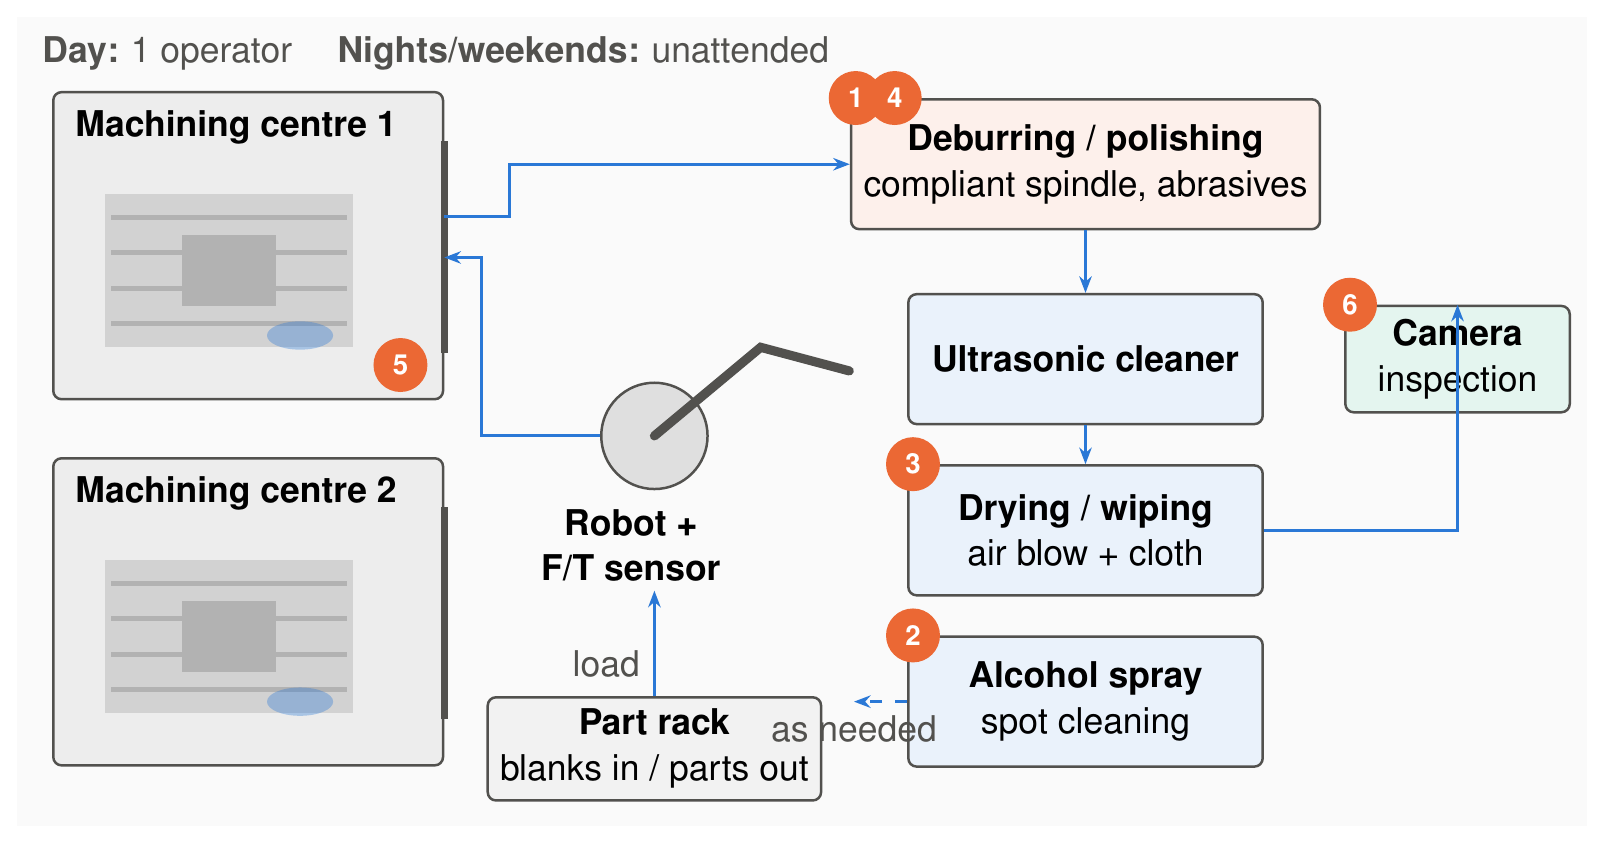
\includegraphics[width=0.535\textwidth]{kimm_factory_cell}\hfill
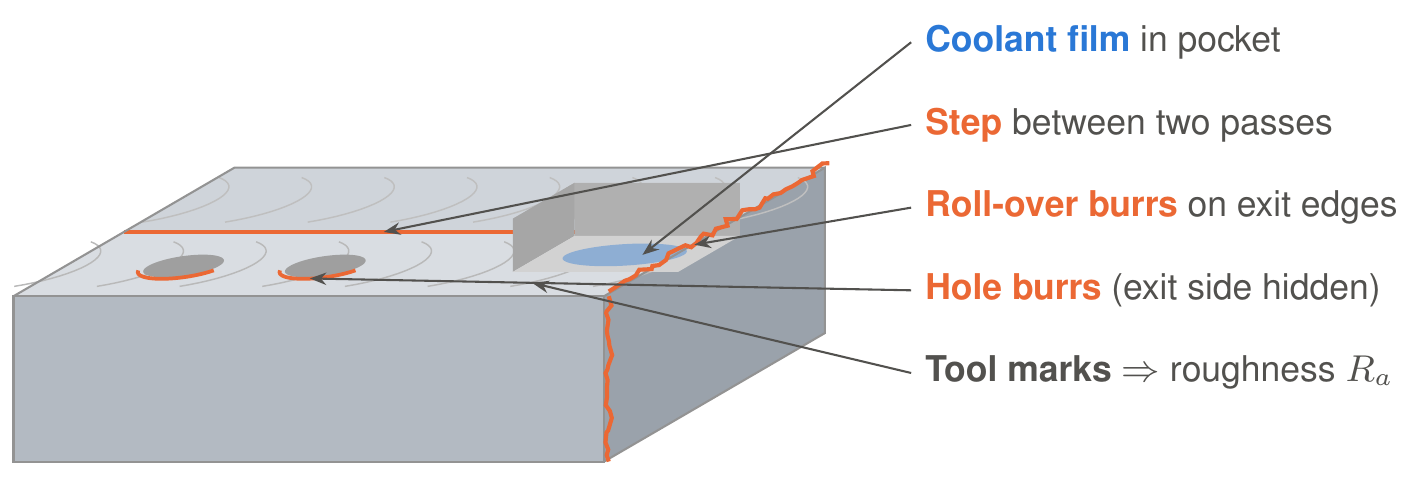
\includegraphics[width=0.445\textwidth]{kimm_part_anatomy}
\caption{(a) Illustrative cell inferred from SOW~\S1, not KIMM's actual layout; orange numbers are the SOW tasks: 1 deburring, 2 alcohol-spray cleaning, 3 drying/wiping after ultrasonic cleaning, 4 step polishing, 5 wiping oil/cutting fluid off the table, 6 camera-lens cleaning.
(b) Schematic machined part showing where each defect type appears.}
\label{fig:setting}
\end{figure}

{\footnotesize
\begin{tabularx}{\textwidth}{@{}P{2.9cm}LP{5.6cm}@{}}
\toprule
\textbf{Task} & \textbf{Goal state (measurable)} & \textbf{Deciding state observable by}\infr \\
\midrule
Deburring & Edge within ISO~13715 call-out ($+a$ burr allowed, $-a$ undercut/chamfer)~\cite{iso13715}; no gouging & 3D vision if burr $\gtrsim$0.1--0.2\,mm; otherwise touch/force \\
Step polishing & Step height and $R_a$ below spec, without form error & Profilometer or hand (haptic); not area cameras \\
Wiping (table; after ultrasonic) & No residual film, full coverage at adequate force & Partly RGB; thin films hard; UV fluorescence for oil~\cite{fraunhofer} \\
Alcohol spray / lens cleaning & Area treated (dosing); image quality restored & Visible contamination; the camera's own image \\
\bottomrule
\end{tabularx}}

\section{What camera + detector can deliver}
\begin{figure}[h]
\centering
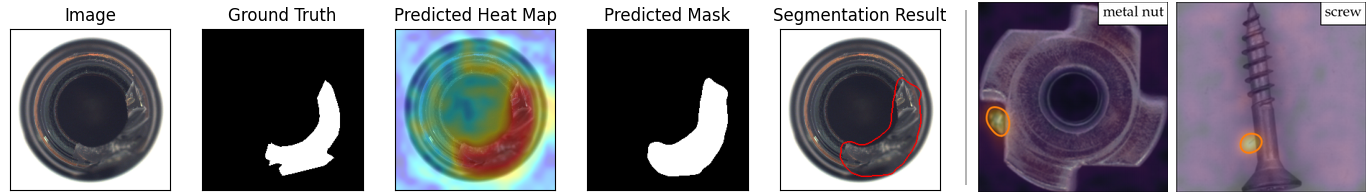
\includegraphics[width=\textwidth]{kimm_detection_io}
\caption{Detector input and outputs.
Left: anomalib PatchCore on an MVTec~AD bottle --- image, ground truth, continuous heatmap, thresholded mask, overlay~\cite{anomalib}.
Right: PatchCore heatmaps on MVTec~AD metal parts~\cite{patchcore}.
Trained on defect-free images only, it flags anything \emph{unusual}, defect or not.}
\label{fig:io}
\end{figure}
\begin{itemize}
\item \textbf{Benchmarks overstate readiness.}
MVTec~AD is saturated (method gaps $<$1 point~\cite{mvtecad2}), yet pixel-AP is only 43--69\% (Fig.~\ref{fig:res}a).
On MVTec~AD~2, SOTA stays below 60\% AU-PRO~\cite{mvtecad2}; the VAND~3.0 winner drops from 53.8 to 51.4\% SegF1 under unseen lighting; dark-field sheet metal reaches 71\%, a shiny can 1.9\% (Fig.~\ref{fig:res}b)~\cite{vand3,robis}.
\item \textbf{Contaminants count as defects.}
On brushed aluminium with a robot camera, 23.5\% of water-stain pixels were flagged; synthetic-stain training cut this to 5.3\% but scratch recall fell 82.6$\to$72.9\%~\cite{stains}.
\item \textbf{Burrs and roughness.} 2D burr detection on reflective joints: AP $\approx$32--45\%~\cite{burr2d}.
Roughness only as grades: 86\% over ISO $R_a$ 0.4--3.2\um~\cite{rough1}; 98.8 vs.\ 76.4\% with/without red--green imaging~\cite{rough2}.
\item \textbf{3D and practice.}
Zivid~One + CAD measured $\approx$0.8\,mm cast burrs comparably to CT~\cite{castburr}; \textmu m features need line profilers (0.4\um{} repeatability over 15\,mm)~\cite{keyence} (Fig.~\ref{fig:res}c).
Industry uses vision to find \emph{edges} and force to absorb magnitude~\cite{fanuc,abbfc}; paint repair places the tool within $\pm$5\,mm, then runs a per-defect recipe~\cite{gm3m}.
\end{itemize}

\begin{figure}[h]
\centering
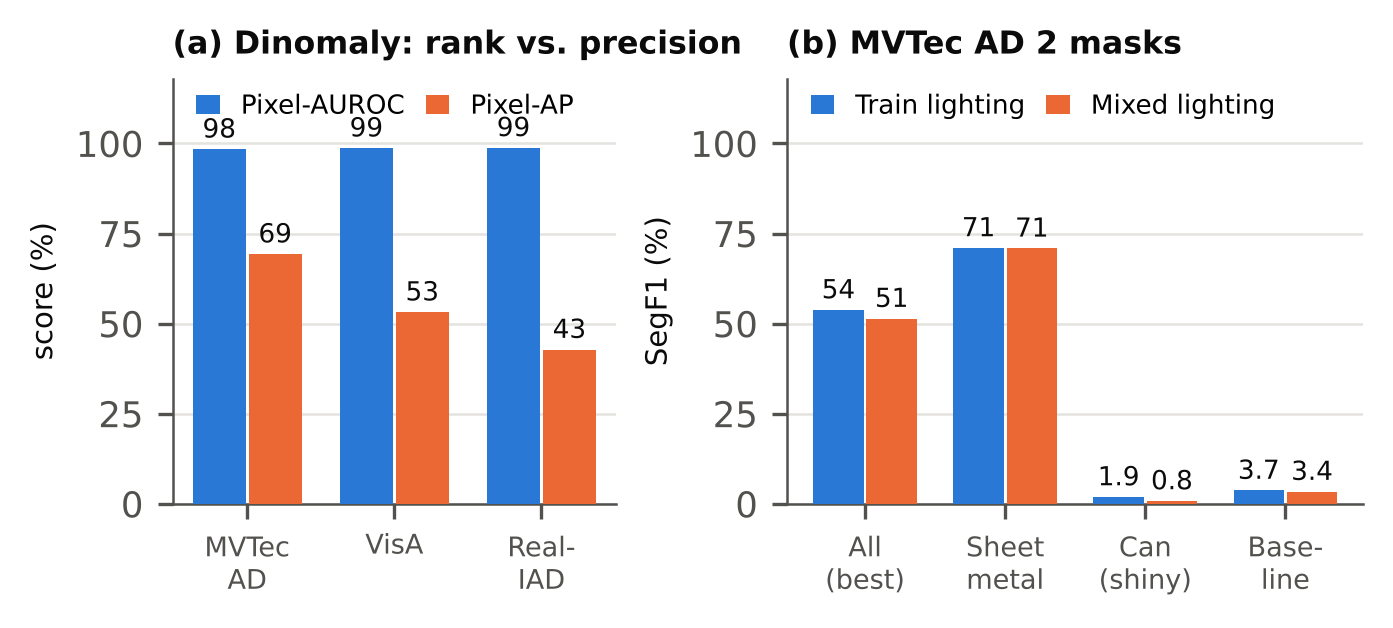
\includegraphics[height=4.75cm]{kimm_heatmap_reliability}\hfill
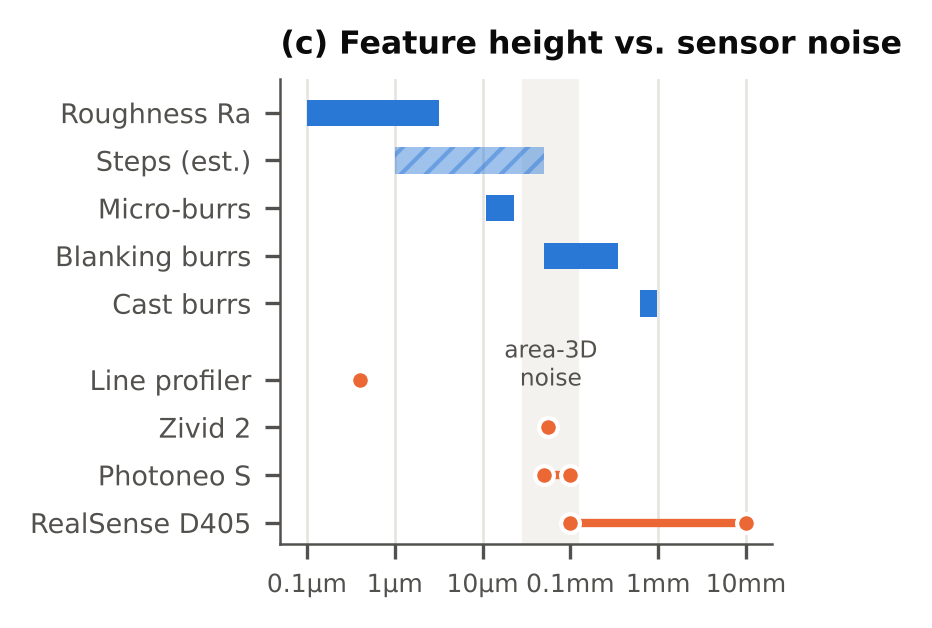
\includegraphics[height=4.75cm]{kimm_scale_vs_sensor}
\caption{(a) Dinomaly ViT-B, multi-class~\cite{dinomaly}.
(b) MVTec~AD~2 SegF1 at each method's threshold~\cite{vand3,robis,mvtecad2}.
(c) Blue: feature heights~\cite{rough1,microburr,brunel,castburr} (hatched = our estimate); orange: sensor depth noise/repeatability, datasheet best case~\cite{keyence,zivid,photoneo,realsense}.}
\label{fig:res}
\end{figure}

\section{Interface to the policy and how to judge it}
\begin{itemize}
\item \textbf{Register the map to the part}, not the image: the tool occludes the defect during contact, so re-render a part-frame map (pose + hand--eye) into the policy's views; run \emph{scan$\to$act$\to$re-scan}.\infr
\item \textbf{The demonstrator must see the same map} (VR/haptic overlay); otherwise actions follow the operator's eyes and the policy learns to ignore the map.\infr
\item \textbf{Metric.}
Removal proxy over tool footprint $A$: $R(\mathbf{x})=\sum_t \tfrac{F_n}{|A|}\|\mathbf{v}\|\,\Delta t\,\mathbf{1}[\mathbf{x}\!\in\!
A(t)]$.
Report defect coverage ($R\ge R_{\min}$), collateral (share of $R$ outside the defect) and, for polishing, $\mathrm{corr}(R,h)$.
Caveats: assumed footprint, mm-level registration, and the $F_z$ fluctuation on our UR10e sensor must be fixed first.
\end{itemize}

\section{Estimating the data requirement without training a policy}
\label{sec:data}
\begin{itemize}
\item \textbf{Scope.}
The SOW excludes policy training and measuring the minimum $N$ for a success rate~\cite{sow}.
Analysis models that score demonstrations are not policies; agree them as ``data-quality indicators'' at the Task-selection review.
\item \textbf{An unconditional VAE action prior is weak.}
It measures motion variety $p(a)$, not how hard $o\!\to\!a$ is; a conditional VAE over action chunks is a policy (ACT).
With 3--6 good demos per condition, its ``stability'' reflects the estimator, and offline losses do not track success~\cite{robomimic}.
\item \textbf{Instead (no policy):} (i) measure cost per successful demo directly (time, failures, retries, reset) per modality --- the solid half of the envelope; (ii) indicators: state--action mutual information from VAE embeddings + k-NN (DemInf, no policy, matches expert quality ratings)~\cite{deminf}, action consistency~\cite{dataquality}, number of strategy modes, observability gap ($R^2$ of actions from vision vs.\ vision + force), demonstrator noise vs.\ tolerance; (iii) saturation curves over 1\ldots$n$ demos give \emph{lower bounds} ($N_{\text{req}}>n$ if not plateaued); split strokes and edge segments to multiply samples; (iv) calibrate on anchors with known $N\!\to$\,success (NRC's prior assistive datasets; robomimic with operator tiers~\cite{robomimic}).
\item \textbf{Express the envelope as} (\#conditions) $\times$ (demos per condition to saturation) $\times$ (cost per demo): per-environment demos saturate while generalization follows a power law in \#environments~\cite{scaling}.
Anchors are less contact-rich than KIMM's tasks; state this limitation.
\end{itemize}

\section{Next steps}
\textbf{Task~1:} score visual observability; pick a pilot pair spanning visual (table wiping) to haptic (deburring or steps).
Hypothesis\infr: the VR--haptic gap widens toward haptic tasks.
\textbf{Task~2:} mock-ups with defects known by construction (or marker/dye) as oracle maps; per modality, log $R(\mathbf{x})$ coverage and the Sec.~\ref{sec:data} indicators.
\textbf{Task~3:} perception requirement plus the calibrated data envelope.
\textbf{Ask KIMM:} materials, finishes and sizes; burr/step ranges and ISO~13715 call-outs; are locations predictable from CAM; existing metrology; lighting control; coolant type.

\vspace{2pt}
{\scriptsize
\renewcommand{\refname}{}\vspace{-1.6em}
\begin{multicols}{2}
\begin{thebibliography}{99}\setlength{\itemsep}{-1pt}\raggedright
\bibitem{sow} KIMM/NRC, SOW v2.0, 21 Aug 2026.
\bibitem{kimmorg} KIMM organization. \url{https://www.kimm.re.kr/eng/sub020101}
\bibitem{kimmko} KIMM Inst.\ of Autonomous Manufacturing. \url{https://www.kimm.re.kr/sub0101}
\bibitem{kcnc} KIMM release, ``Korea's own K-CNC system for machine tools,'' 18 Jun 2025 (via Newswise).
\bibitem{ijat} Kim, Ro, Park, ``Machine Tool Research Trends in Korea,'' IJAT 19(4), 2025.
\bibitem{rogeta} KIMM RoGeTA release, Mar 2026. \url{https://www.kimm.re.kr/eng/sub011001/view/id/1562}
\bibitem{iso13715} ISO 13715:2017, Edges of undefined shape.
\bibitem{fraunhofer} Fraunhofer IPM, fluorescence scanner for residual contamination.
\bibitem{preston} Feng et al., adaptive bonnet polishing (Preston $\Delta Z=KPV\Delta t$), IJAMT 2023.
\bibitem{anomalib} anomalib (Apache-2.0). \url{https://github.com/open-edge-platform/anomalib}
\bibitem{patchcore} Roth et al., PatchCore, CVPR 2022. \url{https://github.com/amazon-science/patchcore-inspection}
\bibitem{mvtecad2} Heckler-Kram et al., MVTec AD 2, arXiv:2503.21622.
\bibitem{vand3} VAND 3.0 challenge report, arXiv:2509.17615.
\bibitem{robis} RoBiS, arXiv:2505.21152.
\bibitem{dinomaly} Guo et al., Dinomaly, CVPR 2025, arXiv:2405.14325.
\bibitem{stains} Surface impurities in visual inspection, arXiv:2501.09579.
\bibitem{burr2d} Tashiro et al., TaylorMade visual burr detection, ICPRAM 2022.
\bibitem{rough1} Metal-machined roughness grades by CNN, ACTA IMEKO 2025.
\bibitem{rough2} Grinding roughness with red--green imaging (VGG16), 2023.
\bibitem{microburr} Burrs in micro-milling Ti-6Al-4V, Eng.\ Proc.\ 111, 2025.
\bibitem{brunel} Benati et al., robot-based burr measurement, Brunel, 1999.
\bibitem{castburr} Mohammed et al., 3D burr detection in castings, J.\ Intell.\ Manuf.\ 34, 2023.
\bibitem{zivid} Zivid 2 specs. \url{https://www.zivid.com/zivid-2-specs}
\bibitem{photoneo} Photoneo MotionCam-3D S specs.
\bibitem{realsense} Intel RealSense D405 specs.
\bibitem{keyence} Keyence LJ-X8060 specs.
\bibitem{fanuc} FANUC intelligent deburring, IMTS 2016.
\bibitem{abbfc} ABB RobotWare Machining Force Control.
\bibitem{gm3m} FANUC case study: GM/3M/Inovision paint repair.
\bibitem{robomimic} Mandlekar et al., robomimic, CoRL 2021, arXiv:2108.03298.
\bibitem{deminf} Hejna et al., Robot data curation with MI estimators (DemInf), RSS 2025.
\bibitem{dataquality} Belkhale, Cui, Sadigh, Data quality in imitation learning, NeurIPS 2023.
\bibitem{scaling} Lin et al., Data scaling laws in imitation learning, ICLR 2025.
\end{thebibliography}
\end{multicols}}
\end{document}
